\documentclass{article}
\usepackage{graphicx} % Required for inserting images
\graphicspath{ {./images/} }
\usepackage[square,numbers]{natbib}
\usepackage[letterpaper,top=2cm,bottom=2cm,left=3cm,right=3cm,marginparwidth=1.75cm]{geometry}
\usepackage{hyperref}

\bibliographystyle{dinat}


\begin{document}


\title{Unit 13}
\author{Chris Hadden}
\date{}
\maketitle

\section{P3 Understand the use of Social Media in business}

\section{Introduction on the use of Social Media in business}
As a valued member of Titanica Media we want you to be able to understand what it is and how we do it. This report will hopefully get you up to speed quickly with our ethos and how we go about business.

When most of our clients want to work with us, they will know from our previous campaigns that they can trust us and that their brand or product will get the boost that they are looking for.

\section{How social media can be used to gather data}
\subsection{Research}
\subsubsection{Primary data}
Primary data is data that in Titanica Media collect ourselves, it's something that we have planned for and we know what we want and what we want to do with the data.
Collecting primary data can be an expensive task so we tend to only do it when there is something we specifically want to find out and there's no other way to get the data.

\subsubsection{Secondary data}
Secondary data is data that was gathered by someone else. This type of data is a lot cheaper the collecting Primary data, but it may not be exactly what we are looking for. Most general data like population density can be found for free, but more specialist Secondary data can be costly. Also as the data is in the public domain other companies may already be using it anc that may reduce it's value to us.

\subsection{Data as a resource}
At Titanica Media we see social media as resource, a resource that we can use to gather data about marketing from.

There are many aspects to gathering social media data that you need to be aware of, some of these are:
\begin{itemize}
\item Data Management: DAMA, a data management professional organization has defined data management as being "The planning, execution and oversite of policies, practices and projects that acquire, control, protect, deliver, and enhance the value of data and information assets.". This defines data management as a set of structures to store data, along with policies to control and collect data. This also goes hand in hand with practices and procedures fo manage how data is used. As you will see this will define the structure of our data management team and our data management system.  \cite{dama}\\
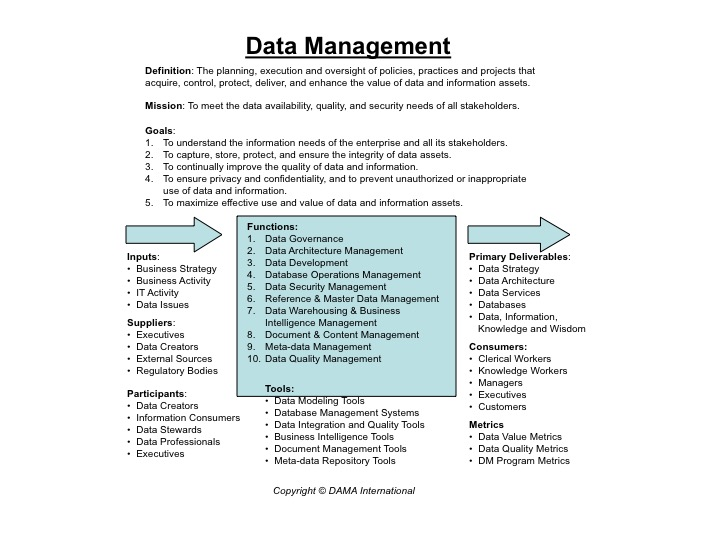
\includegraphics[scale=0.5]{datamanagement} \\
Typically a data management team needs to be setup to deal with how data is organised and stored. 
\item Sources of Data: This is defined as the which is data gathered from social media about users or. This data can be used un many was such as examining relationship status notifications, information about peoples lives, interests, location or socio-economic status. Other data could be gathered from users web cookies or many other inventive ways of gathering it. Gen Z\cite{genz} have grown up with social media. This means they are now an important source of data as they vote, spend money and have opinions. They are very aware of social media and are happy to share information on themselves which is a data goldmine and this data becomes more useful as they become dominant in society.
\item Collection of Data:How we collect data will depend on relationship with the source of data. We can simply record how many times we are mentioned on X \(formerly Twitter \) or we can count the replies on our tweeets. We can also pay for reports and tools supplied by social media such as Hootsuite, X and Facebook that will make our job easier. It depends on what data you need.
\item Analysis of Data: Data Mining is the process of processing all our data collections, which is usually numerous. ALl this social media data make up a data set that shows patterns and trends, anomalies and relationships. There is a semantic difference in the meaning ot pattern and trend here. A pattern will describe the layout of responses and a trend is defined over time. This may not be a geographical layout and may show things like sales across different age ranges for example. There are many factors that can affect how useful the identification of patterns and trends are. This reliability of original data and analysis can affect  the quality of the solutions.
\item Sale of Data: Data is an asset. It can be sold for gain to the company. The extent to which we may gather data is limited by the Data Protection Act in the UK. Thinking of what you personally have been asked to divulge on social media sites will show you how they can collect the data, such as cookies, metrics, clicks etc. Even your IP address can provide details of where you live. This is all valuable to social media sites. It can come from users comments or when they sign up to your site. This data gathering is limited by the Data Protection Act in the UK.

\end{itemize}



\bibliography{bibliography}

\end{document}

